\documentclass[12pt]{article}
\usepackage{amsmath}
\usepackage{fancyhdr}
%\usepackage{lastpage}
\usepackage{hyperref}
\usepackage{amsfonts}
\usepackage[utf8]{inputenc}
\usepackage{amssymb}
\usepackage{listings}
\lstset{
  basicstyle=\small
}
\usepackage[top=1cm, left=2.5cm]{geometry}
\usepackage{color, colortbl}  % farbige Tabellenzellen
\usepackage{tabularx}
\usepackage{hyperref}

\usepackage{graphicx}
\DeclareGraphicsExtensions{.pdf,.png,.jpg}
\renewcommand{\arraystretch}{2}\newcommand{\Jahr}{2014} 
\newcommand{\Semester}{Sommersemester}
\newcommand{\Datum}{\today}
\newcommand{\Semesteranzahl}{2}
\newcommand{\Gesamtsemesterzahl}{2}
\newcommand{\Abschluss}{Bachelor}
\newcommand{\Studienfach}{CES}
\newcommand{\University}{RWTH}
\newcommand{\Nachname}{Klein}
\newcommand{\Vorname}{Lars}
\newcommand{\Strasse}{Friesenstraße}
\newcommand{\Hausnummer}{11}
\newcommand{\PLZ}{52062}
\newcommand{\Ort}{Aachen}
\newcommand{\Email}{lars.klein@rwth-aachen.de}
\newcommand{\Vertrauensdozent}{Prof. Dr. Morgenstern}
%%%%%%%%%%%%%%%%%%%%%%%%%%%%%%%%%%%%%%%%%%%%%%%%%%%%%%%%%%%%%%%%%%%%%
\hypersetup{ 
  pdfauthor   = {\Vorname~\Nachname}, 
  pdfkeywords = {Studienstiftung; KIT; \Vorname~\Nachname}, 
  pdftitle    = {Semesterbericht von~\Vorname~\Nachname~-~\Semester~\Jahr} 
} 

\pagestyle{fancy}
\fancyhf{}
\renewcommand{\headrulewidth}{0pt}
\renewcommand{\footrulewidth}{0pt}
%\fancyfoot[R]{Seite~\thepage~von \pageref{LastPage}}

\definecolor{LightCyan}{rgb}{0.88,1,1}

\pagenumbering{arabic}

\begin{document}

\title{Semesterbericht über das \Semester \Jahr}
\author{\Vorname \Nachname}
\date{\Datum}
\section*{Semesterbericht über das \Semester~\Jahr}
\begin{tabularx}{\textwidth}{@{}llllX}
Name, Vorname:   & \Nachname, \Vorname & Universität         & \University \\
Semesteradresse: &\Strasse~\Hausnummer & Studienfach         & \Studienfach \\
                 &\PLZ~\Ort~~~~~~~     & Semesterzahl        & \Semesteranzahl~von~\Gesamtsemesterzahl \\
                 &                     & Geplanter Abschluss & \Abschluss \\
                 &                     & Vertrauensdozent    & \Vertrauensdozent \\
\end{tabularx}

\begin{large}
\subsection*{Rückblick}
\subsubsection*{Letzte Semester, Vertiefungsrichtungen}
Dieses Semester ist mein sechstes an der RWTH-Aachen. Während dem fünften und sechsten Semester wird der Pflichtteil des Studiums durch relativ frei wählbare Vertiefungsrichtungen ergänzt. CES ist ein grundlagenorientiertes Fach, gerade in Mathematik soll ein fundiertes Basiswissen vermittelt werden. Darauf aufbauend sind viele Vertiefungen möglich. Die einzige wichtige Einschränkung ist, dass man mit der Wahl der Fächer zwei Fachrichtungen abdecken muss. Man könnte also zum Beispiel Mechanik und Verfahrenstechnik vertiefen, darf aber nicht alle Credit-Punkte die zur Verfügung stehen in eine einzige Kategorie investieren.\\
Leider wurden Fächer aus den beiden Richtungen Mathematik und Informatik zu einer gemeinsamen Vertiefungsrichtung zusammengefasst. Dadurch fiel mir die Wahl recht schwer.
Ich würde gerne in die Entwicklung von künstlicher Intelligenz einsteigen, deshalb fand ich den Zwang, eine weitere Vertiefungsrichtung neben Mathematik-Informatik wählen zu müssen, recht unpraktisch.\\
Allerdings gibt es auch in den anderen Fächern interessante Wahlmöglichkeiten. Die Entwicklung autonomer Fahrzeuge ist zum Beispiel auch mechanisch sehr anspruchsvoll.\\
Folgende Fächer habe ich gewählt:\\
\begin{itemize}
\item Data Mining Algorithms
\item Introduction to Neural Networks
\item Elektromechanische Antriebstechnik
\item Foundations of Finite Element Methods
\item Maschinen- und Strukturdynamik
\end{itemize}

Tatsächlich fand ich Data Mining und die Einführung in Neuronale Netze sehr spannend. Data Mining vermittelt Grundlagen zum Speichern und Verwalten von großen Datenmengen, sowie effektive Techniken um neue Erkenntnisse aus diesen Daten zu ziehen. Einige dieser Ansätze wurden auch in der Einführung zu neuronalen Netzen aufgegriffen, glücklicherweise divergierten die beiden Kurse jedoch recht schnell, dadurch gab es nicht allzu viele Überschneidungen. Das Konzept eines künstlichen, neuronalen Netzes hat mich sehr fasziniert. Weil der Kurs an der RWTH allerdings seinem Namen gerecht wird, und wirklich nur eine Einführung darstellt, habe dieses Semester zusammen mit einem Freund einen online-Kurs zu diesem Thema durchgearbeitet. Wir haben auch ein eigenes kleines Framework für das Training von convolutional neural networks gebastelt:

\href{https://bitbucket.org/lhk/cv}{''link to repository''} 

Das Framework funktioniert gut, wir haben zahlreiche unit-tests verwendet, um sicherzustellen, dass der Algorithmus korrekt implementiert wurde.
Allerdings ist die verwendete Programmiersprache recht langsam, für größere Datenmengen und tiefe Netzwerke ist der Code deshalb nicht geeignet.\\

Die beiden anderen Vertiefungsrichtungen waren nicht ganz so faszinierend.
In den ersten beiden Semestern hatten wir die Fächer Mechanik 1 und 2, darin wurden Statik und Dynamik von Festkörpern behandelt. Im vierten Semester folgte darauf Mechanik 3 "Elastostatik". Die Beschreibung von Maschinen- und Strukturdynamik porträtierte das Fach wie eine Art Mechanik 4: "Elastodynamik". Laut Beschreibung sollte darin die Dynamik von komplexen, mehrteiligen Systemen betrachtet werden, inklusive Verformungen.
Das stimmt zwar, weil die Probleme aber so komplex sind, werden simple Ersatzsysteme eingeführt. Diese Ersatzsysteme sind enttäuschend simpel. Eine komplexe Mehrkörpersimulation wurde nicht diskutiert. Tatsächlich werden computergestützte Verfahren nur am Rande erwähnt und sind nicht Teil des eigentlichen Stoffes.\\
Während Maschinen- und Strukturdynamik zwar immerhin noch der Beschreibung, wenn auch nicht den Hoffnungen, gerecht wird, so war Elektromagnetische Antriebstechnik reiner Etikettenschwindel. Eine einzige Vorlesung im gesamten Semester beschäftigt sich mit Motoren. Es gibt keine Modellierung der elektischen Dynamik. Probleme wie Induktion oder Regelung werden nicht angesprochen. Stattdessen beschäftigt sich der gesamte Rest der Vorlesung mit Getrieben: Getriebeanalyse und Getriebesynthese. Die Qualität der Lehre war ausgezeichnet, diese Vorlesung ist für Motorenbauer sicherlich ausgesprochen wichtig, aber man hätte die Veranstaltung doch passender beschreiben können.

\subsubsection{Außerhalb der Uni}
Ein anhaltendes Projekt ist es, neben dem Studium Französisch zu lernen. Dafür habe ich auch dieses Semester an einem e-Tandem des Sprachenzentrum teilgenommen.
Dieser Kurs ist eine Verbindung aus wöchentlichen Gesprächen mit einem französischen Partner und regulärem Unterricht an der RWTH.
Ich hatte großes Glück und habe mich sehr gut mit meinem Partner verstanden.
Neben interessanten politischen Diskussionen, haben wir auch Buch- und Filmempfehlungen ausgetauscht. An dieser Stelle kann ich also einen fantastischen französischen Film weiterempfehlen: "Dinner für Spinner". Es gibt einen typisch amerikanisch-hektischen Remake dieses Films, bitte nur das Original ansehen. Das Lesen von französischen Büchern fiel mir bisher doch recht schwer, durch ständiges Vokabelnachschlagen konnte noch kein angenehmer Lesefluss aufkommen. Aber ich habe eine tolle Entdeckung gemacht: eReader. Leider muss ich hier das Monopol, Amazon, empfehlen. Im Vergleich zu den tolino-Readern, die in vielen Buchhandlungen verkauft werden, hat der Kindle-Reader von Amazon zwei fantastische Vorteile. Man kann nämlich statt dem eingebauten Wörterbuch auch hochwertige Wörterbücher von Drittanbietern im System hinterlegen. Dadurch sind die Übersetzungen viel besser. Außerdem merkt sich das Amazon-System, welche Vokabeln man nachschlagen musste und verfügt über einen integrierten Vokabeltrainer. Damit macht es richtig Spaß, französische Bücher zu lesen. \\
Neben der Fremdsprache habe ich in den vergangenen Semestern versucht, selbstständig Klavier zu lernen. Ein Freund hat mir angeboten, er könne mir Unterricht geben. Diese Bemühungen schliefen aber immer wieder ein, und es war mir peinlich, ihn an die Stunden erinnern zu müssen, zumal sein Studium sehr zeitaufwändig ist. Deshalb habe ich dieses Semester wieder Stunden bei einer professionellen Klavier-Lehrerin genommen. Rückblickend war es ein Fehler, nicht direkt diesen Weg einzuschlagen. Man kommt viel schneller voran, wenn einem ein Profi auf die Finger schaut.

\subsubsection{Hiwi-Job}
Ich habe noch keine klare Vorstellung, in welcher Branche ich nach meinem Studium arbeiten möchte. Die Vorlesung zu neuronalen Netzen hat mich nachhaltig fasziniert, dort wird auch aktiv geforscht. Ich könnte mir also gut vorstellen, nach der Uni an der Uni zu bleiben. Als ersten Schritt in diese Richtung habe ich eine Hiwi-Stelle an unserem Mathe-Institut angenommen, es geht um die Simulation von zwei-Phasen Strömungen in einem Solarkraftwerk. Die Arbeit ist angenehm, vor Allem wegen der ausgesprochen angenehmen Atmosphäre. Meine Bachelor-Arbeit werde ich auch an diesem Institut schreiben.

\pagebreak
\subsection*{Ausblick}
\subsubsection*{Vorlesungsfreie Zeit und Prüfungen}
Teil des siebten Semester ist ein Industrie-Praktikum von 3 Monaten. Ich habe mich bei einer Vielzahl von Unternehmen beworben. Besonders spannend fand ich eine Stelle bei Bayer, dort sollte eine Strömungssimulation zur Entwicklung von Medikamenten angewendet werden. Ich nehme an, dass es um die genaue Berechnung der Resorbtion von Wirkstoffen ging, leider hat Bayer nicht auf meine Bewerbung geantwortet. Das war jedoch Glück, denn durch den online-Kurs in neuronalen Netzen ist erst etwas später meine Begeisterung für dieses Thema erwacht, dazu passt perfekt die Stelle, die ich jetzt als Praktikum gefunden habe: Ich werde bei GE in München arbeiten. Dort soll ich an der Verwendung von neuronalen Netzen für image-classification mitarbeiten. Konkret handelt es sich um die Befundung von MRT- und CT-Aufnahmen. Ich bin begeistert, es handelt sich um grundlagenorientierte Forschung. Ich habe dem Projektleiter ein Paper geschickt, welches mich sehr fasziniert hat und darf nun mehr oder weniger in Eigenregie versuchen, die Ergebnisse des Papers nachzustellen. Darin wird beschrieben, wie man mit Hilfe von interessanten Tricks einen bestimmten Typ von neuronalen Netzen, ein recurrent neural network, welcher sich eigentlich nur für Daten mit Zeit-Dimension eignet, auch für die Klassifizierung von Bildern verwenden kann.
\newline
\newline
\pagebreak
\subsection*{Fazit}
Ich genieße meine Zeit in Aachen. Dank der Vertiefung in Neuronale Netze, kann ich mir bereits vorstellen, wie ich nach der Uni weitermachen könnte.
Momentan freue ich mich vor Allem auf der Frankreich-Aufenthalt mit dem Sprachkurs der Studienstiftung.
\newline
\newline

\subsection*{Noten}
Bisher habe ich immer die aktuellen Noten als eigenen Abschnitt in den Text eingegliedert. Dieser Bericht umfasst aber zwei Semester, außerdem wurde der Vertrauensdozent gewechselt. Deshalb hänge ich meinen gesamten Notenspiegel an das Dokument an.
\bigskip
\\
\Ort, \Datum\\
\\
\Vorname~\Nachname
\\
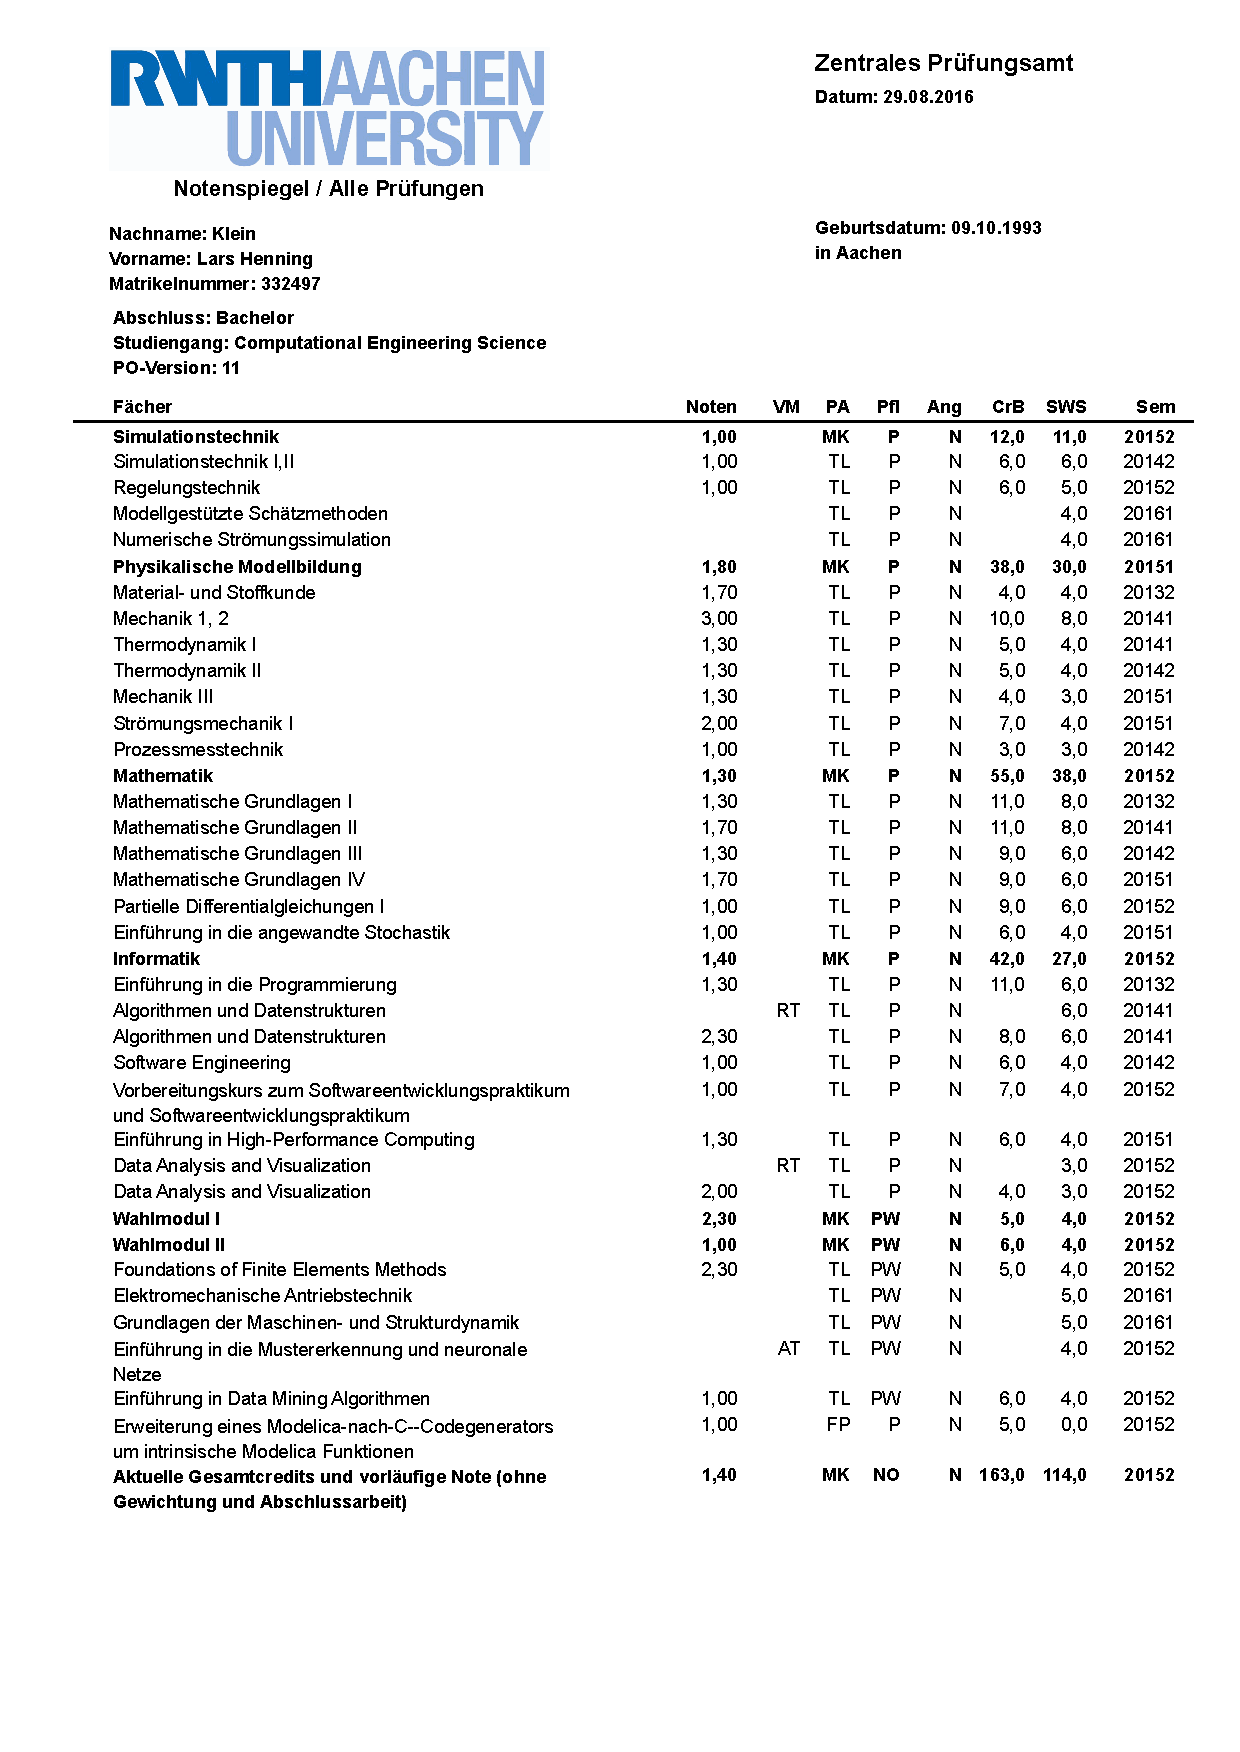
\includegraphics[width=500pt]{Notenspiegel}


\end{large}

\end{document}
